\section{Evola on Spanish Falangism}

\begin{wrapfigure}{rt}{.3\textwidth}
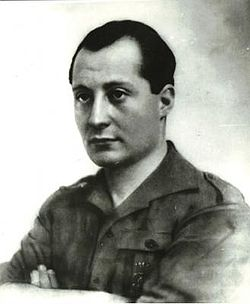
\includegraphics[width=.25\textwidth]{JoseAntonio-DeRivera.jpg}
\end{wrapfigure}

José Antonio Primo de Rivera was executed by the Spanish left on November 20, 1936. Although we are a day late because we were only recently provided with the Italian text, we will provide this translation of Evola's evaluation of the Spanish Falangists. Intended for the general public, it was published in January 1937 in \textbf{Tratto da Lo Stato}. It was subsequently included in the book \textbf{Fascismo e Terzo Reich} (``Fascism and the Third Reich'').

Please see \textit{What is Spanish Falangism}\footnote{\url{http://www.gornahoor.net/?page_id=1202}} for the translated text.

\begin{quotex}
We believe that the state does not have to justify its behaviour at every turn, just as no individual or social class does, in so far as it holds to a guiding principle all the time. All the while the state is made out to be God by Rousseau's idea that the state, or the will of those it represents, is always right. What makes the state like God is the belief that the will of the state, embodied by absolute monarchs in the past and now by the popular vote, is always right. The monarch may have erred; the popular vote may err because neither truth nor goodness derives from an act or assertion of the will. Goodness and truth are perennial tributaries of reason, and to ascertain whether one is in the right it is not enough to ask the king---whose dictate seemed always just to his supporters---nor enough to canvass the people---whose decision is always right according to the disciples of Rousseau. What must be done rather is to verify whether our actions and our thoughts are in agreement at every step with a permanent aspiration.

\flright{\textsc{José Antonio Primo de Rivera}}
\end{quotex}


Julius Evola takes the opportunity to express his own ideas on counter-revolution, under the pretext of evaluating the program of the Spanish Falangists from the later part of the 1930s. First of all, he points out that a political soldier must understand the cause for which he is fighting. Ideas, not blind action, are the driving forces behind historical change. Thus, he would seem to support the publication of manifestos or programs and be opposed to the helter-skelter approach of a destructive revolution under the hope of trying to pick up the pieces.

The same applies to nationalism. Beyond any concrete manifestation, a nation is at its base a spiritual reality, that is, ``a predestined, cosmic unity.'' Therefore, it cannot base itself on materialist categories such as race or territorial boundaries. Evola then digresses from this ``particularism'' and subtly brings up the idea of Empire as itself being a supranational spiritual reality. The Falangist state, therefore, is radically opposed to the liberal, secular, ``night watchman'' state.

As spiritual reality, the state is organic and results from ``cells'': the family, the local community, and common business and professional associations. It is hierarchical and opposes any class conflict.

After defining the state, the Falangists deal with the individual. Once again, Evola notes the Traditional idea of the Person: free, autonomous, ordered to eternal life, an absolute value in himself. The Person's freedom is legitimized from above and is opposed to individualistic self-assertion.

The Falange is opposed to materialism. Any movement based on biological determinism or race, and justified by empirical science is not a valid counter-revolutionary movement. They attach themselves to the Catholic faith, in reality, the only historical religion of Spain. Evola here comes very close the the Hermetic view of the Catholic religion. He sees in it a relation to the Primordial Tradition (the so-called ``Church of John'') while simultaneously entertaining an anti-clericalism (``the Church of Peter''). Evola concludes with a positive evaluation of the Falange.

One sees in this that Evola, despite himself, is really of the \textbf{Old Right}. He sees the Europe before the French Revolution as sane and normal. He also writes approvingly of the masters of the Old Right, from Joseph de Maistre, to Donoso Cortes to José Antonio Primo de Rivera. Any group claiming to be based on ``Evola'' needs to always keep the principles enunciated in his review in mind.

\flrightit{Posted on 2010-11-21 by Cologero}

\begin{center}* * *\end{center}

\begin{footnotesize}
\begin{sffamily}
\texttt{Will on 2011-01-10 at 14:06 said:}

There is some great footage of Jose Antonio, as well as general information about the Falange, here in this documentary:

\url{http://www.youtube.com/watch?v=yzum\_CU44jk}


\end{sffamily}
\end{footnotesize}

